\documentclass[11pt,a4paper]{article}

\usepackage{fontspec}
\setmainfont{TeX Gyre Termes}
\setsansfont{TeX Gyre Heros}
\setmonofont{DejaVu Sans Mono}[Scale=0.88]

\usepackage[a4paper,top=25mm,bottom=25mm,left=27mm,right=27mm,headheight=24pt]{geometry}
\usepackage{amsmath,amssymb,mathtools,bm}
\usepackage[table]{xcolor}
\usepackage{graphicx}
\usepackage{booktabs}
\usepackage{tabularx}
\usepackage{array}
\usepackage{enumitem}
\usepackage{float}
\usepackage{subcaption}
\usepackage{caption}
\usepackage{fancyhdr}
\usepackage{listings}
\usepackage{microtype}
\usepackage{titlesec}
\usepackage{hyperref}
\usepackage{xurl}

\definecolor{AcademicBlue}{HTML}{1D4E89}
\definecolor{TableGray}{HTML}{F1F1F1}
\definecolor{Rule}{HTML}{B8B8B8}
\definecolor{CodeBg}{HTML}{F5F5F5}

\hypersetup{
  colorlinks=true,
  linkcolor=AcademicBlue,
  urlcolor=AcademicBlue,
  citecolor=AcademicBlue,
  pdftitle={Multi-view Gaussian Initialization from Dense 3D Geometry},
  pdfauthor={Zepeng Chu},
  pdfsubject={Technical Report},
  pdfkeywords={3D Gaussian Splatting, initialization, dense geometry, LoG, PCA}
}

\graphicspath{{assets/}}
\captionsetup{font=small,labelfont=bf,labelsep=quad}
\captionsetup[subfigure]{font=footnotesize,labelfont=bf,justification=centering}
\setlist{nosep,leftmargin=2em}
\setlength{\parindent}{1.5em}
\setlength{\parskip}{0pt}
\setlength{\emergencystretch}{2em}
\linespread{1.08}
\renewcommand{\arraystretch}{1.18}
\newcolumntype{Y}{>{\raggedright\arraybackslash}X}
\newcolumntype{R}{>{\raggedleft\arraybackslash}X}

\titleformat{\section}
  {\Large\bfseries}
  {\thesection}{0.7em}{}
\titleformat{\subsection}
  {\large\bfseries}
  {\thesubsection}{0.7em}{}
\titlespacing*{\section}{0pt}{2.2ex plus .5ex}{1.1ex}
\titlespacing*{\subsection}{0pt}{1.8ex plus .4ex}{.8ex}

\pagestyle{fancy}
\fancyhf{}
\fancyhead[L]{\footnotesize\itshape Multi-view Gaussian Initialization from Dense 3D Geometry}
\fancyhead[R]{\footnotesize Zepeng Chu}
\fancyfoot[C]{\small\thepage}
\renewcommand{\headrulewidth}{0.4pt}
\renewcommand{\headrule}{\hbox to\headwidth{\color{Rule}\leaders\hrule height \headrulewidth\hfill}}
\fancypagestyle{plain}{
  \fancyhf{}
  \fancyfoot[C]{\small\thepage}
  \renewcommand{\headrulewidth}{0pt}
}

\lstdefinestyle{reportcode}{
  backgroundcolor=\color{CodeBg},
  basicstyle=\ttfamily\small,
  frame=single,
  rulecolor=\color{Rule},
  framerule=0.5pt,
  breaklines=true,
  columns=fullflexible,
  keepspaces=true,
  showstringspaces=false,
  xleftmargin=0.4em,
  xrightmargin=0.4em,
  aboveskip=0.8em,
  belowskip=0.8em
}

\newcommand{\methodid}{\texttt{dense\_lab\_log\_ellipse\_grid\_region\_pca}}
\newcommand{\code}[1]{\texttt{#1}}

\begin{document}
\pagenumbering{arabic}
\thispagestyle{plain}

\begin{center}
  \vspace*{-8mm}
  {\LARGE\bfseries Multi-view Gaussian Initialization from Dense 3D Geometry\par}
  \vspace{5pt}
  {\large From 2D Perceptual Regions to Anisotropic 3D Gaussians\par}
  \vspace{10pt}
  {\normalsize Zepeng Chu\par}
  \vspace{3pt}
  {\small Technical Report\par}
  {\small Version 1.0\par}
  {\small July 2026\par}
  \vspace{3pt}
  {\footnotesize Method identifier: \methodid\par}
\end{center}
\vspace{6pt}

\begin{abstract}
We present a region-level method for initializing anisotropic 3D Gaussians from pixel-aligned dense 3D geometry. Instead of lifting every pixel into an independent Gaussian, the method first identifies image regions with meaningful structure or spatial coverage, extracts a single continuous 3D surface support from each region, and estimates Gaussian position, orientation, and scale through principal component analysis (PCA).

The 2D proposal stage has two complementary branches. Multichannel, multiscale Laplacian of Gaussian (LoG) detection in Lab space identifies luminance and chromatic structure, while a structure tensor expands each keypoint into an orientation-adaptive ellipse. A regular grid supplements low-texture surfaces that LoG does not adequately cover. Both proposal types share the same 3D continuity test, PCA validity checks, and multi-view fusion procedure. Fusion jointly constrains position, covariance, normal, scale, and color, thereby avoiding merges based on spatial proximity alone.

On 48 views of the Tanks and Temples Truck scene, the complete VGGT and region-initialization pipeline reaches 26.89\,dB PSNR and 0.9057 SSIM after 30,000 optimization steps, compared with 23.67\,dB and 0.7932 for the COLMAP sparse pipeline under the same gsplat settings. This single-scene pipeline-level comparison indicates higher training-view reconstruction quality and faster convergence under the evaluated configuration.

\noindent\textbf{Keywords:} 3D Gaussian Splatting; dense 3D geometry; Laplacian of Gaussian; structure tensor; PCA; multi-view fusion
\end{abstract}

\medskip
\noindent\rule{\textwidth}{0.5pt}
\medskip

\section{Problem Formulation and Design Goals}

Given $V$ views, the method expects the following pixel-aligned data:

\begin{lstlisting}[style=reportcode]
processed_images:      [V, H, W, 3]
world_points:          [V, H, W, 3]
processed_valid_mask:  [V, H, W]
\end{lstlisting}

The objective is to construct a set of anisotropic Gaussians that can be loaded directly into a 3D Gaussian Splatting optimizer~\cite{kerbl2023gaussians}. In the reported experiments, Gaussian optimization and differentiable rasterization are implemented with gsplat~\cite{ye2025gsplat}. The input geometry may be supplied by a system such as VGGT~\cite{wang2025vggt} or reconstructed on demand from depth, camera intrinsics, and extrinsics. The initializer does not require confidence values and is therefore not tied to a particular dense reconstruction method.

Per-pixel lifting and uniform point sampling have three principal drawbacks:

\begin{enumerate}
  \item nearby pixels on the same local surface produce many redundant primitives;
  \item uniform sampling does not distinguish the representational needs of structured and low-texture regions; and
  \item multi-view observations repeatedly represent the same surface, while distance-only fusion may cross thin objects or occlusion boundaries.
\end{enumerate}

We instead use the following region-level formulation:

\begin{equation}
\boxed{
\begin{gathered}
\text{2D perceptual region}\rightarrow\text{continuous 3D surface support}\\
\rightarrow\text{anisotropic Gaussian proposal}\rightarrow\text{multi-view fusion}
\end{gathered}}
\label{eq:pipeline}
\end{equation}

\section{Method}

\subsection{Multichannel, Multiscale LoG in Lab Space}

The RGB image is first converted to normalized CIE Lab coordinates:

\begin{equation}
L\leftarrow L/100,\qquad a\leftarrow a/128,\qquad b\leftarrow b/128.
\end{equation}

For channel $c\in\{L,a,b\}$ and scale $\sigma$, we compute a scale-normalized LoG response:

\begin{equation}
R_c(x,y;\sigma)=\sigma^2\Delta\left(G_\sigma*I_c\right)(x,y).
\end{equation}

Each channel is robustly normalized with a single median absolute deviation (MAD) computed across all valid pixels and all scales. The normalized channel responses are then fused as

\begin{equation}
\widehat R_c=\frac{R_c}{\operatorname{MAD}(R_c)+\varepsilon},\qquad
S=\sqrt{\widehat R_L^2+w_c\widehat R_a^2+w_c\widehat R_b^2}.
\label{eq:log-fusion}
\end{equation}

The current scale set is $\sigma\in\{1.0,1.6,2.5,4.0,6.4,10.0\}$. Guard scales at both ends participate in comparison but do not generate final candidates. A candidate must be a strict local maximum in a $3\times3\times3$ neighborhood of $(x,y,\sigma)$, so position and characteristic scale are selected jointly.

\begin{figure}[htbp]
  \centering
  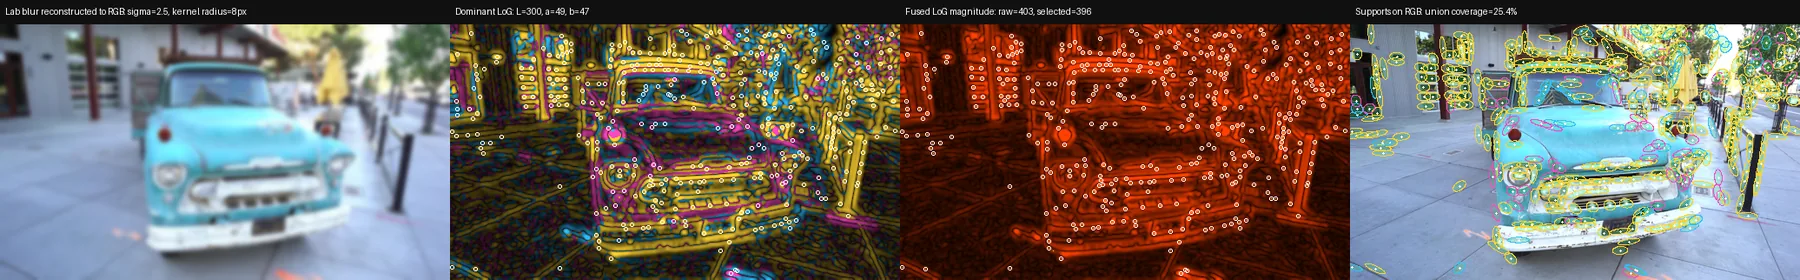
\includegraphics[width=\textwidth]{log-sampling-sigma-2p5.png}
  \caption{Generated Lab-LoG sampling visualization. The panels show the input image, Gaussian-blurred image, fused response, and candidate regions projected back onto the original image.}
  \label{fig:log-sampling}
\end{figure}

\subsection{Structure-Tensor Ellipses and Within-Scale Merging}

LoG localizes image structure, while a multichannel structure tensor determines its local orientation and shape:

\begin{equation}
J=G_\rho*\sum_{c\in\{L,a,b\}}w_c
\begin{bmatrix}
I_{c,x}^2&I_{c,x}I_{c,y}\\
I_{c,x}I_{c,y}&I_{c,y}^2
\end{bmatrix},
\qquad \rho=1.5\sigma.
\label{eq:structure-tensor}
\end{equation}

After eigendecomposition of $J$, the strong-gradient direction becomes the ellipse's short axis and the weak-gradient direction becomes its long axis. The base radius is $2.5\sigma$, and the maximum axis ratio is 4. Rather than discarding nearby candidates with greedy NMS, the method connects compatible ellipses at the same scale using IoU, orientation, Lab color, and 3D continuity. A replacement ellipse is then fitted by matching the second moments of the union. The merged region must still satisfy area and shape constraints.

\begin{figure}[htbp]
  \centering
  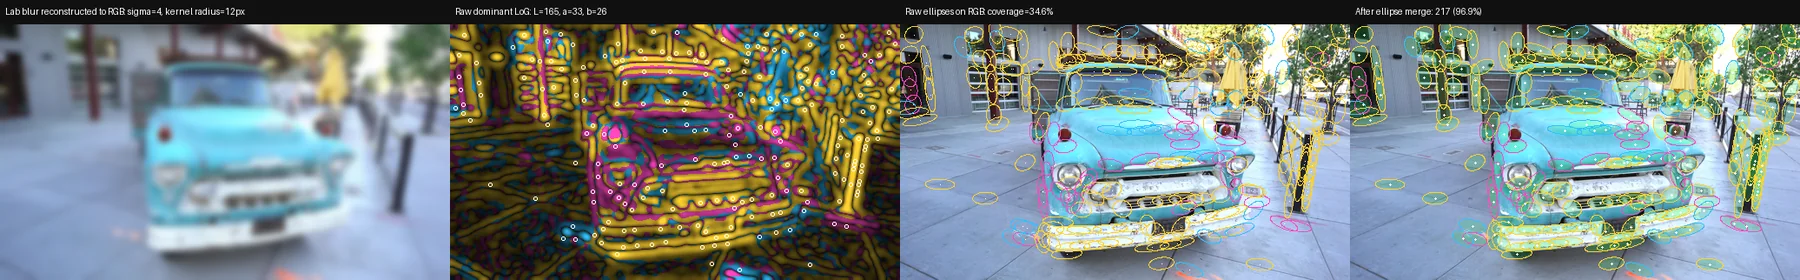
\includegraphics[width=\textwidth]{ellipse-merge-sigma-4.png}
  \caption{Generated within-scale candidates and ellipse-merging result. Merging preserves the joint support of compatible candidates instead of retaining only the strongest center.}
  \label{fig:ellipse-merge}
\end{figure}

\subsection{Regular-Grid Completion for Low-Texture Regions}

LoG naturally favors locations with chromatic or textural variation. To cover floors, walls, and other nearly uniform surfaces, the image is partitioned into $12\times12$ pixel cells. Any sufficiently valid cell not completely covered by the structural ellipses enters the supplementary candidate set. Once selected, all valid pixels in the cell are used; the ellipse mask is not subtracted pixel by pixel.

Adjacent cells grow only through the 4-neighborhood. A merge requires similar median Lab color and 3D continuity for at least 60\% of valid pixel pairs along the shared boundary. Every proposed component is also checked for holes, a maximum of 1,500 support pixels, and a convex-hull fill ratio of at least 0.9. These constraints prevent narrow, winding, or strongly non-convex regions.

\begin{figure}[htbp]
  \centering
  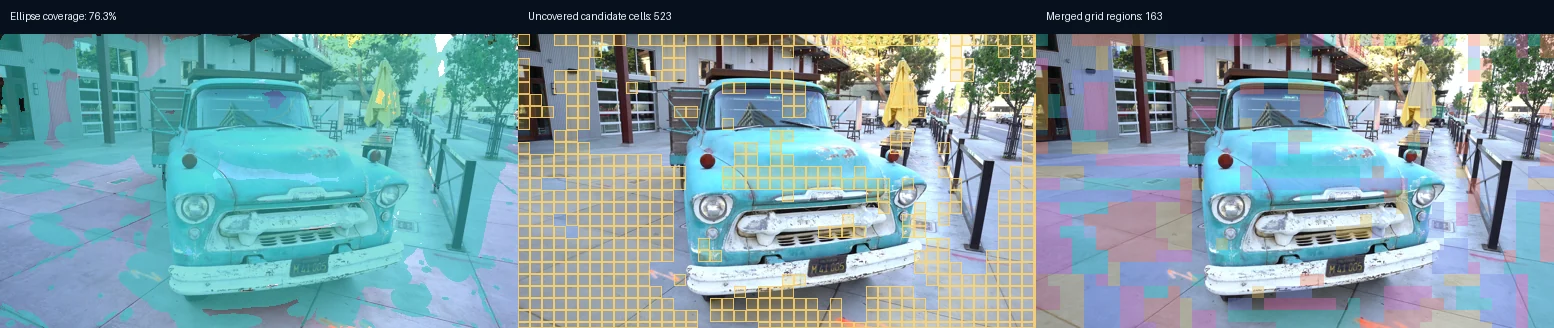
\includegraphics[width=\textwidth]{grid-supplement-view1.png}
  \caption{Structural-ellipse coverage, incompletely covered grid candidates, and approximately convex region growing. Grid regions and structural ellipses enter the same downstream 3D fitting procedure.}
  \label{fig:grid-supplement}
\end{figure}

\subsection{View-Level 3D Continuity}

Adjacent image pixels may lie on opposite sides of an occlusion boundary. For each view, the method estimates a typical 3D distance per image pixel from all valid 8-neighborhood edges:

\begin{equation}
s_{\mathrm{ref}}=\operatorname{median}_{(i,j)}
\frac{\lVert P_i-P_j\rVert_2}{\lVert p_i-p_j\rVert_2}.
\end{equation}

Two neighboring pixels are considered surface-continuous only if

\begin{equation}
\frac{\lVert P_i-P_j\rVert_2}{\lVert p_i-p_j\rVert_2}
\le 3s_{\mathrm{ref}}.
\label{eq:continuity}
\end{equation}

This threshold is fixed for the complete view rather than relaxed independently by each local region. The same test is used for path checks between ellipse centers, continuity along shared grid boundaries, and connected-component extraction inside every region.

A structural ellipse retains the connected component containing its LoG center pixel, whose 3D point remains the Gaussian center. A grid region has no distinguished keypoint, so it retains its largest connected component and uses the 3D centroid of that component.

\subsection{PCA Parameterization}

For the retained 3D support points $\{P_i\}$, the covariance and its eigendecomposition are

\begin{equation}
\Sigma=\frac1N\sum_i(P_i-\mu)(P_i-\mu)^\mathsf T,
\qquad
\Sigma=Q\operatorname{diag}(\lambda_1,\lambda_2,\lambda_3)Q^\mathsf T.
\label{eq:pca}
\end{equation}

The activated Gaussian scales are $s_i=\sqrt{\lambda_i}$, and $Q$ is converted to a unit quaternion in \code{wxyz} order. A fit must contain at least two meaningful principal directions, enforced by $\lambda_2/\lambda_1\ge0.01$. Line-like degeneracies are rejected, while thin planar regions may retain a small normal eigenvalue. Nearly ideal planar grid regions receive a finite normal-thickness floor to prevent zero-thickness rendering and optimization instabilities.

RGB color is converted to zeroth-order spherical harmonics as

\begin{equation}
\mathrm{SH}_{\mathrm{DC}}=\frac{\mathrm{RGB}-0.5}{0.28209479177387814}.
\end{equation}

Initial opacity is 0.2. The initialization file stores activated scales and activated opacities; the training model converts them to log-scales and opacity logits when loading.

\subsection{Multi-view Similarity-Graph Fusion}

Voxels are used only to retrieve nearby proposal pairs, never to average all proposals in the same voxel. Two proposals receive a similarity-graph edge only if all of the following conditions hold:

\begin{itemize}
  \item squared Mahalanobis distance under their average covariance is at most 9;
  \item the normal-angle difference is at most $30^\circ$;
  \item the maximum corresponding principal-scale ratio is at most 3; and
  \item the Lab color difference is at most 20.
\end{itemize}

The position condition is

\begin{equation}
d_M^2=(\mu_i-\mu_j)^\mathsf T
\left(\frac{\Sigma_i+\Sigma_j}{2}+\varepsilon I\right)^{-1}
(\mu_i-\mu_j).
\label{eq:mahalanobis}
\end{equation}

Each connected component of the similarity graph is fused by second-moment matching:

\begin{equation}
\mu=\frac1K\sum_k\mu_k,
\qquad
\Sigma=\frac1K\sum_k
\left[\Sigma_k+(\mu_k-\mu)(\mu_k-\mu)^\mathsf T\right].
\label{eq:moment-fusion}
\end{equation}

The fused covariance is subjected to PCA and geometric validity checks again. If fusion produces an invalid result, the original proposals in that component are retained rather than deleting the complete component.

\section{Initialization Statistics}

Table~\ref{tab:init-stats} summarizes the resulting initialization on the 48-view Truck scene.

\begin{table}[htbp]
  \centering
  \caption{Initialization statistics for the 48-view Truck scene.}
  \label{tab:init-stats}
  \small
  \begin{tabularx}{\textwidth}{@{}Y r Y@{}}
    \toprule
    \textbf{Stage} & \textbf{Count} & \textbf{Description} \\
    \midrule
    LoG / ellipse regions & 158,457 & Final structural regions across all views \\
    Grid candidate cells & 26,428 & Valid cells not completely covered by ellipses \\
    Grid regions & 8,942 & After appearance, continuity, and convexity checks \\
    Total 2D regions & 167,399 & Sum of ellipse and grid regions \\
    Valid ellipse proposals & 96,387 & Passed 3D support and PCA validation \\
    Valid grid proposals & 5,337 & Passed 3D support and PCA validation \\
    Proposals before fusion & 101,724 & Region acceptance rate of 60.8\% \\
    Compatible graph edges & 235,573 & From 910,948 retrieved candidate pairs \\
    Merged components & 10,320 & In addition to 33,600 singleton components \\
    Fallback components & 9 & Invalid fused geometry; original proposals retained \\
    \rowcolor{TableGray}
    Final Gaussians & \textbf{43,948} & A 56.8\% reduction relative to pre-fusion proposals \\
    \bottomrule
  \end{tabularx}
\end{table}

The structural ellipses cover approximately 77.3\% of valid image pixels. Grid-support pixels may overlap ellipse regions, so their support cannot be added directly to the ellipse coverage and interpreted as total coverage.

\section{Experiments}

\subsection{Experimental Setup}

\begin{table}[htbp]
  \centering
  \caption{Pipeline-comparison setup.}
  \label{tab:experiment}
  \small
  \begin{tabularx}{\textwidth}{@{}>{\raggedright\arraybackslash}p{38mm}Y@{}}
    \toprule
    \textbf{Item} & \textbf{Setting} \\
    \midrule
    Dataset and scene & Tanks and Temples~\cite{knapitsch2017tanks}, Truck \\
    Input sequence & 48 images uniformly selected from 251 frames \\
    Processed resolution & $518\times294$ \\
    Dense geometry & VGGT~\cite{wang2025vggt}, pixel-aligned world coordinates \\
    Comparison pipeline & COLMAP~\cite{schoenberger2016sfm} sparse, PINHOLE, same processed images, no undistortion \\
    COLMAP reconstruction & 48/48 registered images and 8,487 sparse points \\
    Optimizer & Identical gsplat~\cite{ye2025gsplat} training, loss, learning-rate, and densification settings \\
    Training & 30,000 steps, random seed 42, final SH degree 3 \\
    Evaluation & Every 500 steps over all 48 optimization views \\
    \bottomrule
  \end{tabularx}
\end{table}

The experiment compares two complete pipelines:

\begin{enumerate}
  \item \textbf{VGGT plus region initialization:} VGGT dense geometry $\rightarrow$ the proposed method $\rightarrow$ gsplat;
  \item \textbf{COLMAP sparse:} COLMAP cameras and sparse points $\rightarrow$ isotropic three-neighbor initialization $\rightarrow$ gsplat.
\end{enumerate}

Both pipelines use the same 48 input images and identical gsplat optimization settings, enabling a direct comparison of initial quality, convergence, and final reconstruction quality for the complete workflows.

\subsection{Initial Rendering}

\begin{figure}[htbp]
  \centering
  \begin{subfigure}[t]{0.32\textwidth}
    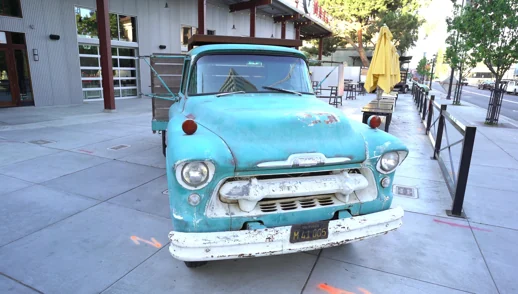
\includegraphics[width=\linewidth]{target-view1.png}
    \caption{Reference image}
  \end{subfigure}\hfill
  \begin{subfigure}[t]{0.32\textwidth}
    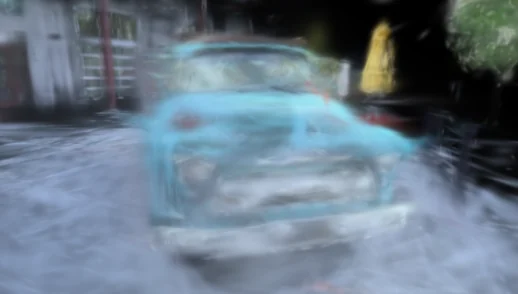
\includegraphics[width=\linewidth]{init-vggt-view1.png}
    \caption{Proposed pipeline}
  \end{subfigure}\hfill
  \begin{subfigure}[t]{0.32\textwidth}
    
\includegraphics[width=\linewidth]{init-colmap-view1.png}
    \caption{COLMAP sparse}
  \end{subfigure}
  \caption{Rendering comparison before optimization.}
  \label{fig:initial-render}
\end{figure}

Before optimization, the proposed pipeline reaches 11.47\,dB PSNR compared with 10.92\,dB for COLMAP. Their SSIM values are 0.3966 and 0.3862, and their L1 errors are 0.1962 and 0.2388, respectively. The initial L1 error is therefore reduced by approximately 17.9\%. Qualitatively, the dense region-based initialization already covers the truck body and large background surfaces. Step zero remains visibly blurred and semi-transparent because each Gaussian initially carries only a DC color term.

\subsection{Convergence and Final Results}

\begin{table}[htbp]
  \centering
  \caption{Quantitative results over all 48 optimization views.}
  \label{tab:results}
  \small
  \begin{tabularx}{\textwidth}{@{}Y R R R@{}}
    \toprule
    \textbf{Metric} & \textbf{VGGT + region init.} & \textbf{COLMAP sparse} & \textbf{Difference} \\
    \midrule
    Initial PSNR & 11.47\,dB & 10.92\,dB & +0.55\,dB \\
    Initial SSIM & 0.3966 & 0.3862 & +0.0105 \\
    Initial L1 & 0.1962 & 0.2388 & $-17.9\%$ \\
    Steps to 25\,dB & 12,000 & Not reached by 30,000 & --- \\
    \rowcolor{TableGray}
    30k PSNR & \textbf{26.89\,dB} & 23.67\,dB & \textbf{+3.22\,dB} \\
    \rowcolor{TableGray}
    30k SSIM & \textbf{0.9057} & 0.7932 & \textbf{+0.1125} \\
    \rowcolor{TableGray}
    30k L1 & \textbf{0.0241} & 0.0382 & \textbf{$-37.1\%$} \\
    \bottomrule
  \end{tabularx}
\end{table}

\begin{figure}[H]
  \centering
  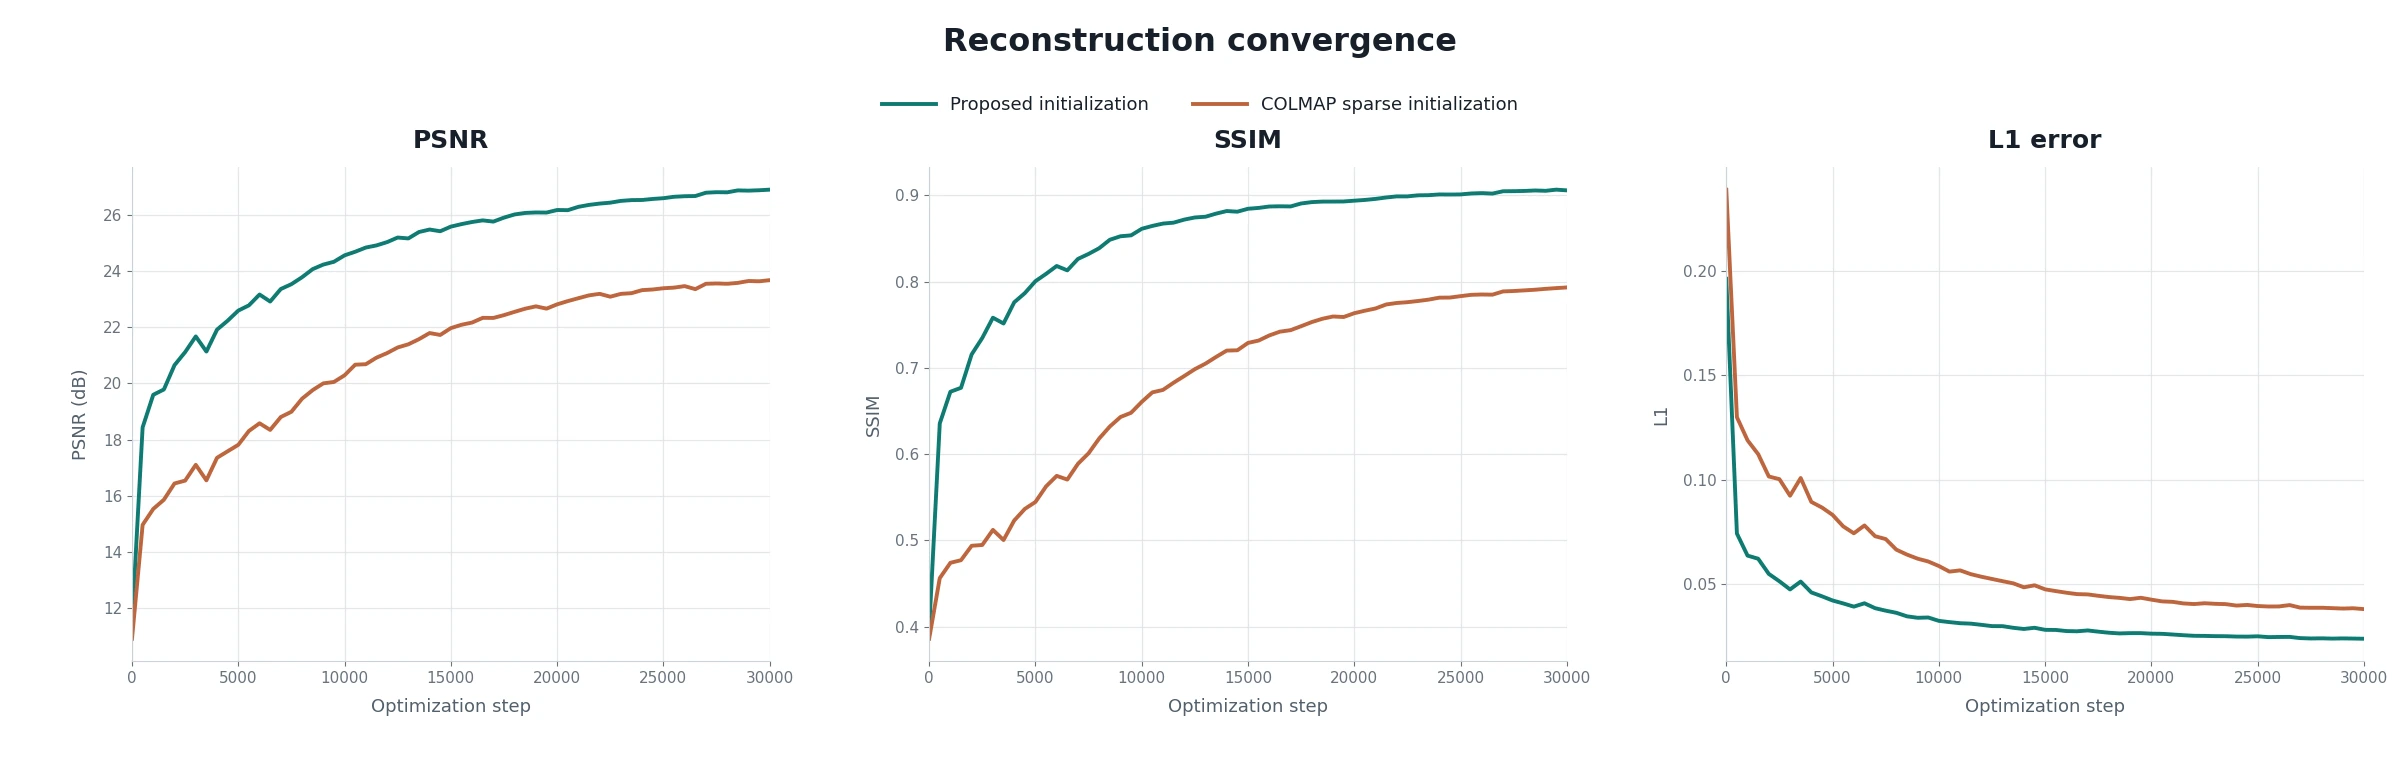
\includegraphics[width=0.95\textwidth]{convergence.png}
  \caption{PSNR, SSIM, and L1 curves over all 48 views used for optimization. The proposed pipeline reaches higher reconstruction quality earlier under the current setup.}
  \label{fig:convergence}
\end{figure}

\begin{figure}[H]
  \centering
  \begin{subfigure}[t]{0.32\textwidth}
    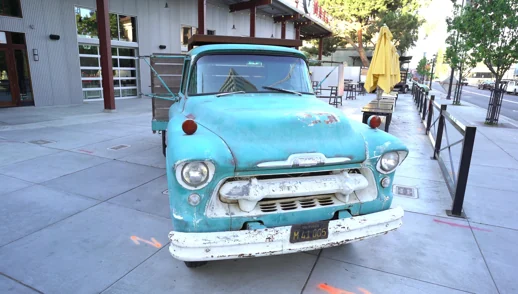
\includegraphics[width=\linewidth]{target-view1.png}
    \caption{Reference image}
  \end{subfigure}\hfill
  \begin{subfigure}[t]{0.32\textwidth}
    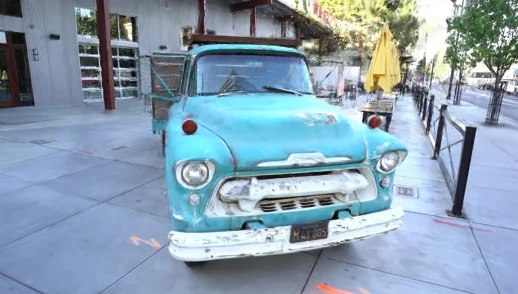
\includegraphics[width=\linewidth]{final-vggt-view1.png}
    \caption{Proposed pipeline, 30k}
  \end{subfigure}\hfill
  \begin{subfigure}[t]{0.32\textwidth}
    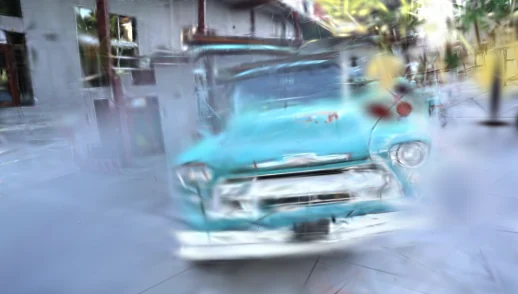
\includegraphics[width=\linewidth]{final-colmap-view1.png}
    \caption{COLMAP, 30k}
  \end{subfigure}
  \caption{Rendered results after 30,000 training steps.}
  \label{fig:final-render}
\end{figure}

The complete VGGT plus region-initialization pipeline achieves higher all-view reconstruction quality and reaches 25\,dB after 12,000 steps; the COLMAP pipeline does not reach that threshold within 30,000 steps. Initial quality, convergence curves, and final metrics consistently show that dense geometry combined with structure-aware region initialization provides a more effective starting point and a better final reconstruction on the Truck scene.

\section{Scope and Limitations}

The current evaluation is limited to a single scene and reports metrics on
the same 48 views used for optimization. The comparison is conducted at the
complete-pipeline level: the proposed pipeline uses VGGT dense geometry,
whereas the baseline uses COLMAP sparse geometry. Consequently, the current
experiment does not independently isolate the contribution of the region
initialization method from that of the input geometry source. Broader
multi-scene evaluation and controlled initialization ablations are left for
future work.

\section{Conclusion}

This work reformulates Gaussian initialization from point sampling into local surface-region modeling. Lab-LoG and the structure tensor identify image structure, while regular grids complete low-texture coverage. A fixed view-level 3D continuity test extracts a single surface from each 2D region, PCA converts that support into an anisotropic Gaussian with physically meaningful orientation and scale, and a multi-attribute similarity graph removes multi-view redundancy.

On the 48-view Truck scene, the complete pipeline achieves better initial quality, faster convergence, and higher training-view reconstruction quality than the evaluated COLMAP sparse pipeline under the same gsplat optimization settings.

\begin{thebibliography}{9}

\bibitem{kerbl2023gaussians}
B. Kerbl, G. Kopanas, T. Leimk\"uhler, and G. Drettakis,
``3D Gaussian Splatting for Real-Time Radiance Field Rendering,''
\emph{ACM Transactions on Graphics}, vol.~42, no.~4, 2023.
\url{https://repo-sam.inria.fr/fungraph/3d-gaussian-splatting/}

\bibitem{ye2025gsplat}
V. Ye, R. Li, J. Kerr, M. Turkulainen, B. Yi, Z. Pan, O. Seiskari,
J. Ye, J. Hu, M. Tancik, and A. Kanazawa,
``gsplat: An Open-Source Library for Gaussian Splatting,''
\emph{Journal of Machine Learning Research}, vol.~26, no.~34, pp.~1--17, 2025.
\url{https://www.jmlr.org/papers/v26/24-1476.html}

\bibitem{wang2025vggt}
J. Wang, M. Chen, N. Karaev, A. Vedaldi, C. Rupprecht, and D. Novotny,
``VGGT: Visual Geometry Grounded Transformer,''
in \emph{Proceedings of the IEEE/CVF Conference on Computer Vision and Pattern Recognition},
pp.~5294--5306, 2025.
\url{https://openaccess.thecvf.com/content/CVPR2025/html/Wang_VGGT_Visual_Geometry_Grounded_Transformer_CVPR_2025_paper.html}

\bibitem{knapitsch2017tanks}
A. Knapitsch, J. Park, Q.-Y. Zhou, and V. Koltun,
``Tanks and Temples: Benchmarking Large-Scale Scene Reconstruction,''
\emph{ACM Transactions on Graphics}, vol.~36, no.~4, 2017.
\url{https://www.tanksandtemples.org/}

\bibitem{schoenberger2016sfm}
J. L. Sch\"onberger and J.-M. Frahm,
``Structure-from-Motion Revisited,''
in \emph{Proceedings of the IEEE Conference on Computer Vision and Pattern Recognition},
pp.~4104--4113, 2016.
\url{https://doi.org/10.1109/CVPR.2016.445}

\end{thebibliography}

\end{document}
